\subsection{Semantic segmentation}
For this problem, the use of semantic segmentation was priorized. We uses fully convolutional network to achieve our semantic segmentation. One of the main problem of this task, is that the output need to have the same dimensions as the input. So the tricks to uses max pooling to reduce the dimension of the image while incresasing the number of channel is more challenging, since a we need to apply a upsampling technique in the network. We try two architecture, one of them uses the max pooling with the upsampling and the other one keep the same dimensions along the network. 
\\
Another challenge that we add in this task, was to deal with the presence of the class imbalance. We try to have loss function that were meaningful for this task and that take this challenge into account. We mainly try two types of loss function.
\\
Like it was discuss in the dataset section, the amount of data was problematic for training our model. We then uses the technique of data augmentation that still make sens for the type of image that we wanted to apply the semantic segmentation on.
\\
Finally, we discuss about the training details that we uses for our FCN.

\subsubsection{Architecture}
The first architecture that was tried is a network called U-Net. The name of this network is due to his shape. This net apply max pooling to reduce the dimensions of the feature map while increasing the number of channel to obtain more expressivity. Four max pooling are applied. After, there is four upsampling that are applied. The dimension of the feature map is then increased while the number of channel is decreased. The upsampling can either be learn or it can be an interpolation. The particularity of U-Net is the uses of skip connection. The skip connection are between the the same dimension feature map before each max pooling and after each upsampling. Those skip connection help to learn how to upsample well the image. A little difference with the figure \ref{fig:unet} of the architecture, we used padding on our convolution filter, so the dimensions on the encoder part and the decoder part are the same and no croping is needed. \\

The second architecture that was used is the VGG 16 pretrained with batch norm. We wanted to use a pretrained net because of the low amount of image that we had. This net was built do to image classification, so some modification was needed to adapt it for our task. The max pooling were removed from the net, so the input stay the same size as the output.
 
\begin{figure}[H]
	\centering
	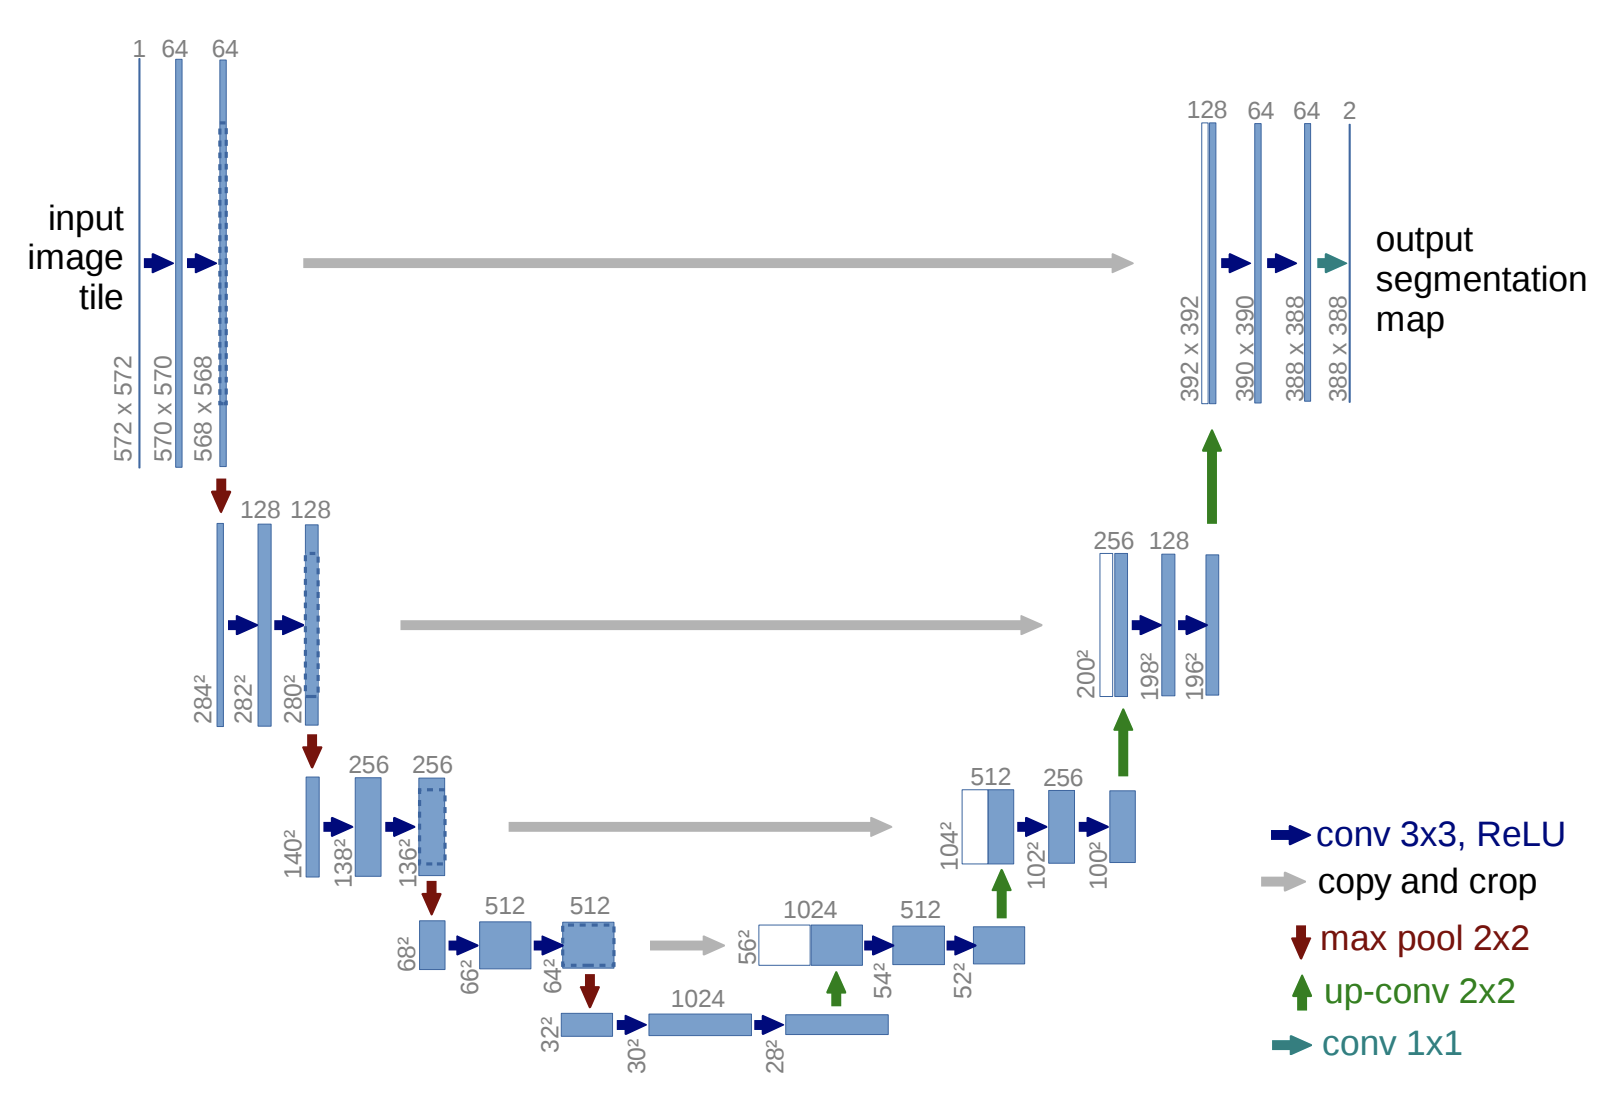
\includegraphics[width=7.5cm,height=6cm]{figures/unet-architecture.png}
	\caption{U-Net architecture.}
	\label{fig:unet}
\end{figure}

Furthermore, we kept only the first seven layer of the net. This is mainly due to time computation constraint. A last layer of convolution with kernel size of one was added to the net the have nine channel in output of the net, like our task. 

\subsubsection{Loss function}
As describe earlier, for our model to learn the task, we needed to have a loss function that isn't too much influenced by the class that are more present in the image. Details such as line and face-off dot are as important as the ice. We started by using the cross entropy loss. In this loss, each pixel is given an equal proportion in the loss, so the class that are more present in a batch, will have a bigger impact on the loss. We adjust the weight in the loss function with a formula base on the proportion of the class in the batch as discussed in this paper \cite{Paszke}. \\
\\
The second loss function that was used is the dice loss. This loss is calculated for each class and the means on all class is taken afterwards. Here is the formula of the loss.
\begin{gather*}
 \frac{1}{nb\_class}*\sum\limits_{i=1}^{nb\_class}\Big(1-\frac{2\sum\limits_{pixels}y_{true}y_{pred}}{\sum\limits_{pixels}y_{true}^{2}+\sum\limits_{pixels}y_{pred}^{2}}\Big)
\end{gather*}
This has the particularity to give to each class the same proportion in the loss. This was usefull for recognizing all the class.

\subsubsection{Data augmentation}
The number of image that we label for our task was not enough to properly train our model for a lot on epoch. Also the labeling task was quite time consuming so that's mainly why we were not able to extract a large amount of data (only 43 images). A way to increase our training data set was to do data augmentation. Since we didn't have a lot of image, we didn't want to apply data augmentation that would modify to much the semantic of the image. We wanted our new image to be as realistic as possible of want a hockey ring look like. We decided to apply an horizontal rotation. As it can be seen it the figure \ref{fig:flip} the new image is a image that is possible in the sense of hockey broadcast. This allow us to double the amount of image available for training. 
\begin{figure}[H]
	\centering
	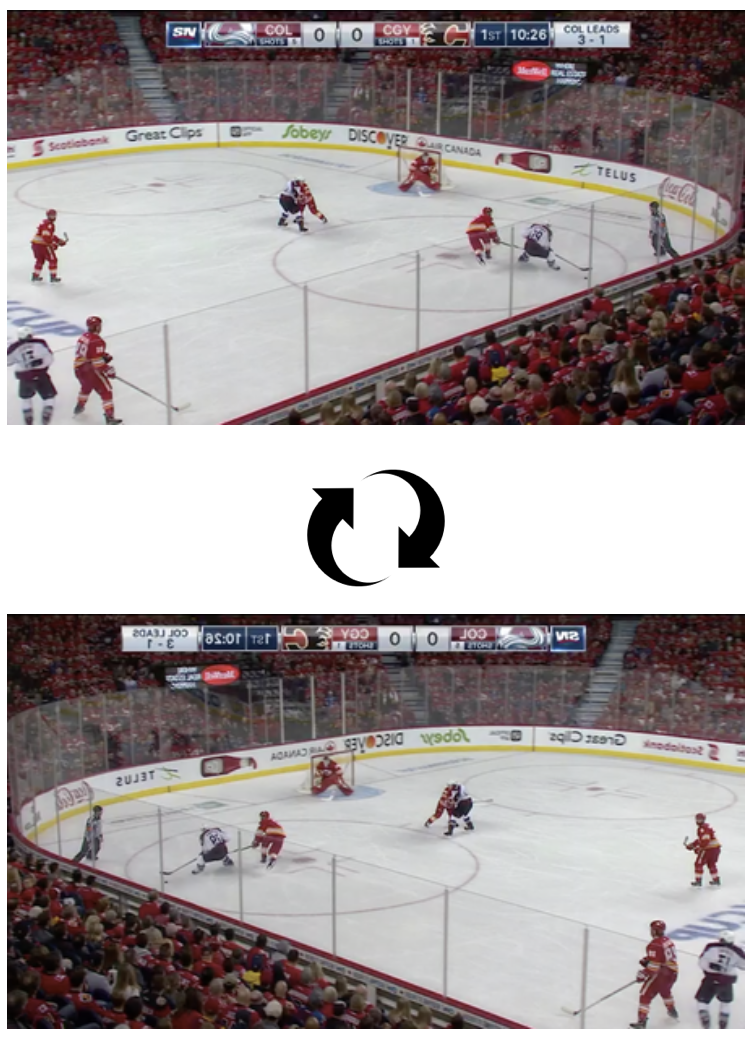
\includegraphics[width=7cm,height=8cm]{figures/rotation-example.png}
	\caption{Horizontal rotation}
	\label{fig:flip}
\end{figure}

\subsubsection{Training details}
For the training of our models, we uses a kind of grid search approach with some parameters that we were changing each time. A challenge that we add was that we needed to look at image prediction each time to see if our model was converging well. Since we add 9 classes and didn't had a good and representative measure of accuracy we were not able to rely only on the lowest loss value. Sometimes, the loss was low, but the class were not well predicted and few of them was actually predicted. It happends that with higher loss, we were more satisfy of the result of the prediction on either the training set and the test set. So it was not possible to do a full grid search and take the combination of parameters that gave the lowest loss. 
\\
We tried to vary the learning rate, the batch size, the model uses, the loss uses, the weight apply on the cross entropy, the optimizer, whether we uses learned upsampling method on the U-Net or interpolation, the number of epoch and whether normalize the image according to the normalization calculated on imagenet. Our best result is presented in the result section. 

\subsection{Mapping to 2D plan}
The goal of this projet is then to map the image of hockey broadcast in a 2D plan. To do so, a good representation of the ice rink feature must be learn by our algorithm. There is some key point in a hockey ring that are always at the same spot and that is really usefull to map the image in a plan. For example, the joint between the line and the board is an important feature. Be positioning the well recognized pixel on the true pixel value in the 2D map, it's possible to find the good deformation to apply to the image. As for now, we hadn't try anything related to the mapping. This would be try more thoroughly when our model of semantic segmentation will performed better. 
